\chapter{Encuesta de Aceptación del Bachillerato en la Población}

En los primeros días de marzo de 2011, por medio del gobierno del municipio de Irapuato, se levantaron 1000 encuestas aleatorias entre la población para conocer el grado de aceptación del proyecto. A continuación se presentan los resultados obtenidos.

\section{Resultados de la Encuesta}

Los resultados de la encuesta se muestran en las siguientes páginas.

\clearpage
\subsection{Nivel Educativo}

El nivel escolar de los encuestados es el siguiente:

\begin{figure}[h!]
	\centering
	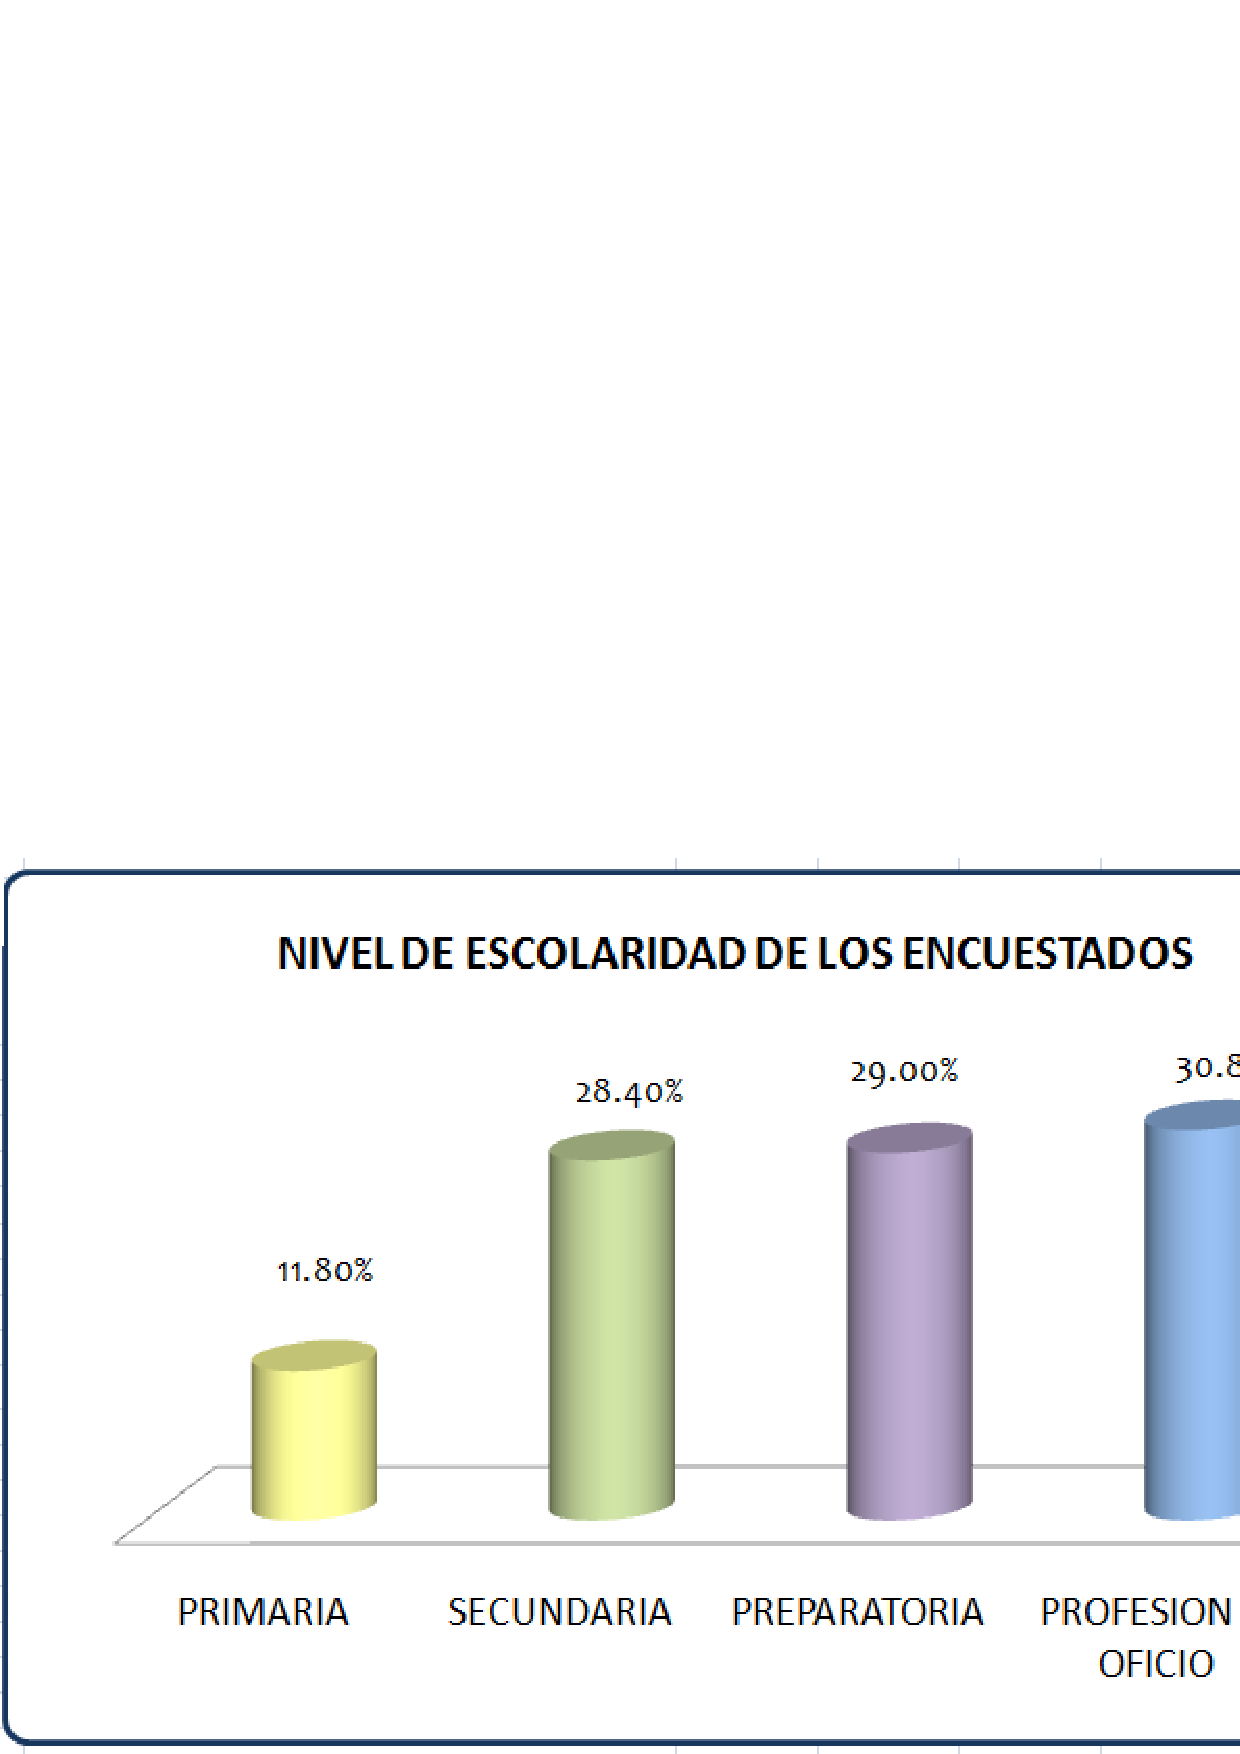
\includegraphics[scale=0.5]{images/encuesta_nivel_educativo}
	\caption{Nivel Educativo de los Encuestados. Fuente: Elaboración Propia.}
	\label{fig:Encuesta:NivelEducativo}
\end{figure}

\begin{table}[h!]
    \caption{Nivel Educativo}
    \label{tbl:Encuesta:NivelEducativo}
    \centering
    \begin{tabular}{l|r@{.}l@{\%}}
	    \multicolumn{1}{c|}{Escolaridad} &
	    	\multicolumn{2}{c}{Porcentaje} \\
	    \hline
	    \hline
	    Primaria           & 11 & 80 \\
	    Secundaria         & 28 & 40 \\
	    Preparatoria       & 29 & 00 \\
	    Profesional/Oficio & 30 & 80 \\
	    \hline
	    \multicolumn{3}{l}{\footnotesize Fuente: Elaboración Propia, 2011.}
    \end{tabular}
\end{table}


\clearpage
\subsection{Necesidad Percibida del Instituto}

La opinión de si es necesario o no la creación del instituto es la siguiente:

\begin{figure}[h!]
	\centering
	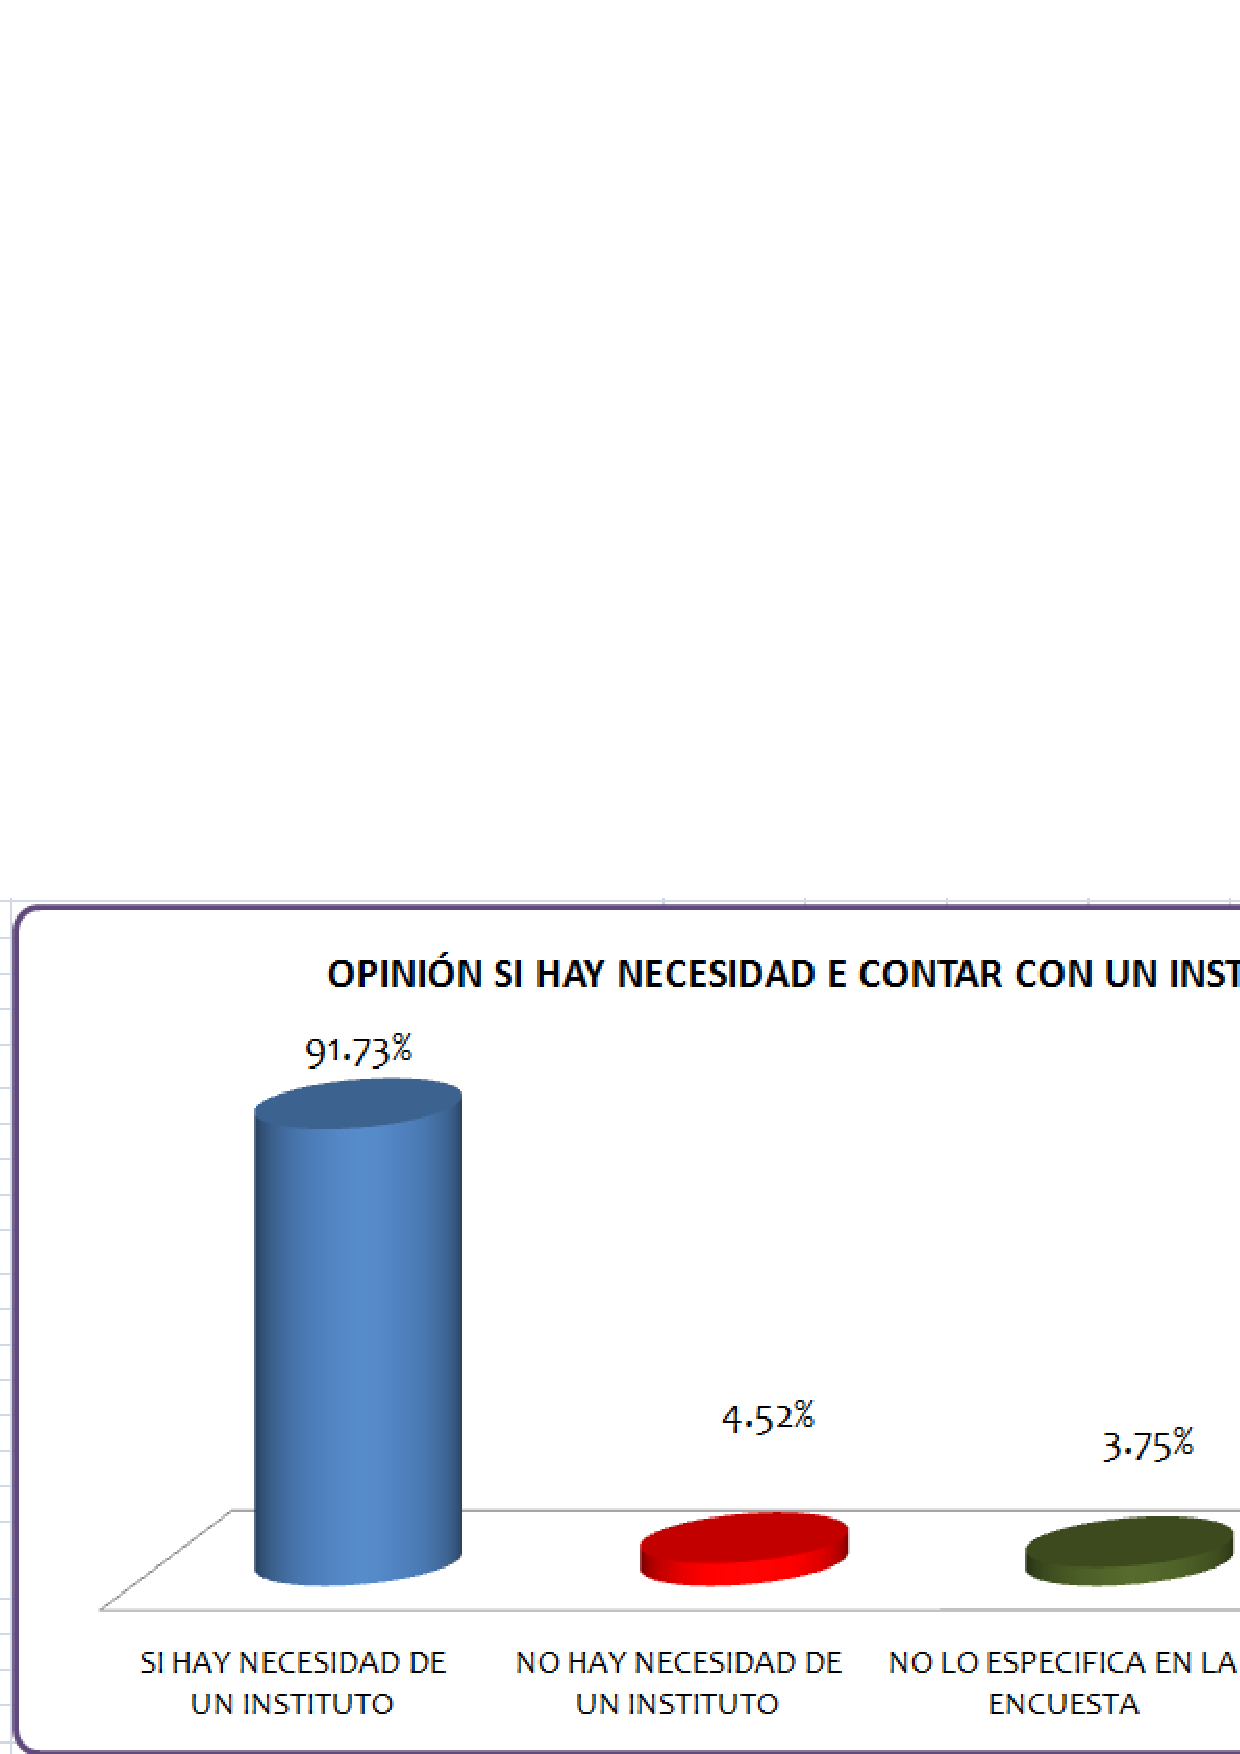
\includegraphics[scale=0.5]{images/encuesta_necesidad}
	\caption{Necesidad de Crear el Instituto. Fuente: Elaboración Propia.}
	\label{fig:Encuesta:Necesidad}
\end{figure}

\begin{table}[h!]
    \caption{Necesidad Percibida del Instituto}
    \label{tbl:Encuesta:Necesidad}
    \centering
    \begin{tabular}{l|r@{.}l@{\%}}
	    \multicolumn{1}{c|}{Respuesta Dada} &
	    	\multicolumn{2}{c}{Porcentaje} \\
	    \hline
	    \hline
	    Sí hay necesidad del instituto   & 91 & 73 \\
	    No hay necesidad del instituto   &  4 & 52 \\
	    No lo especifica en la respuesta &  3 & 75 \\
	    \hline
	    \multicolumn{3}{l}{\footnotesize Fuente: Elaboración Propia, 2011.}
    \end{tabular}
\end{table}


\clearpage
\subsection{Carreras Técnicas}

Las carreras técnicas que se consideraron necesarias fueron:

\begin{figure}[h!]
	\centering
	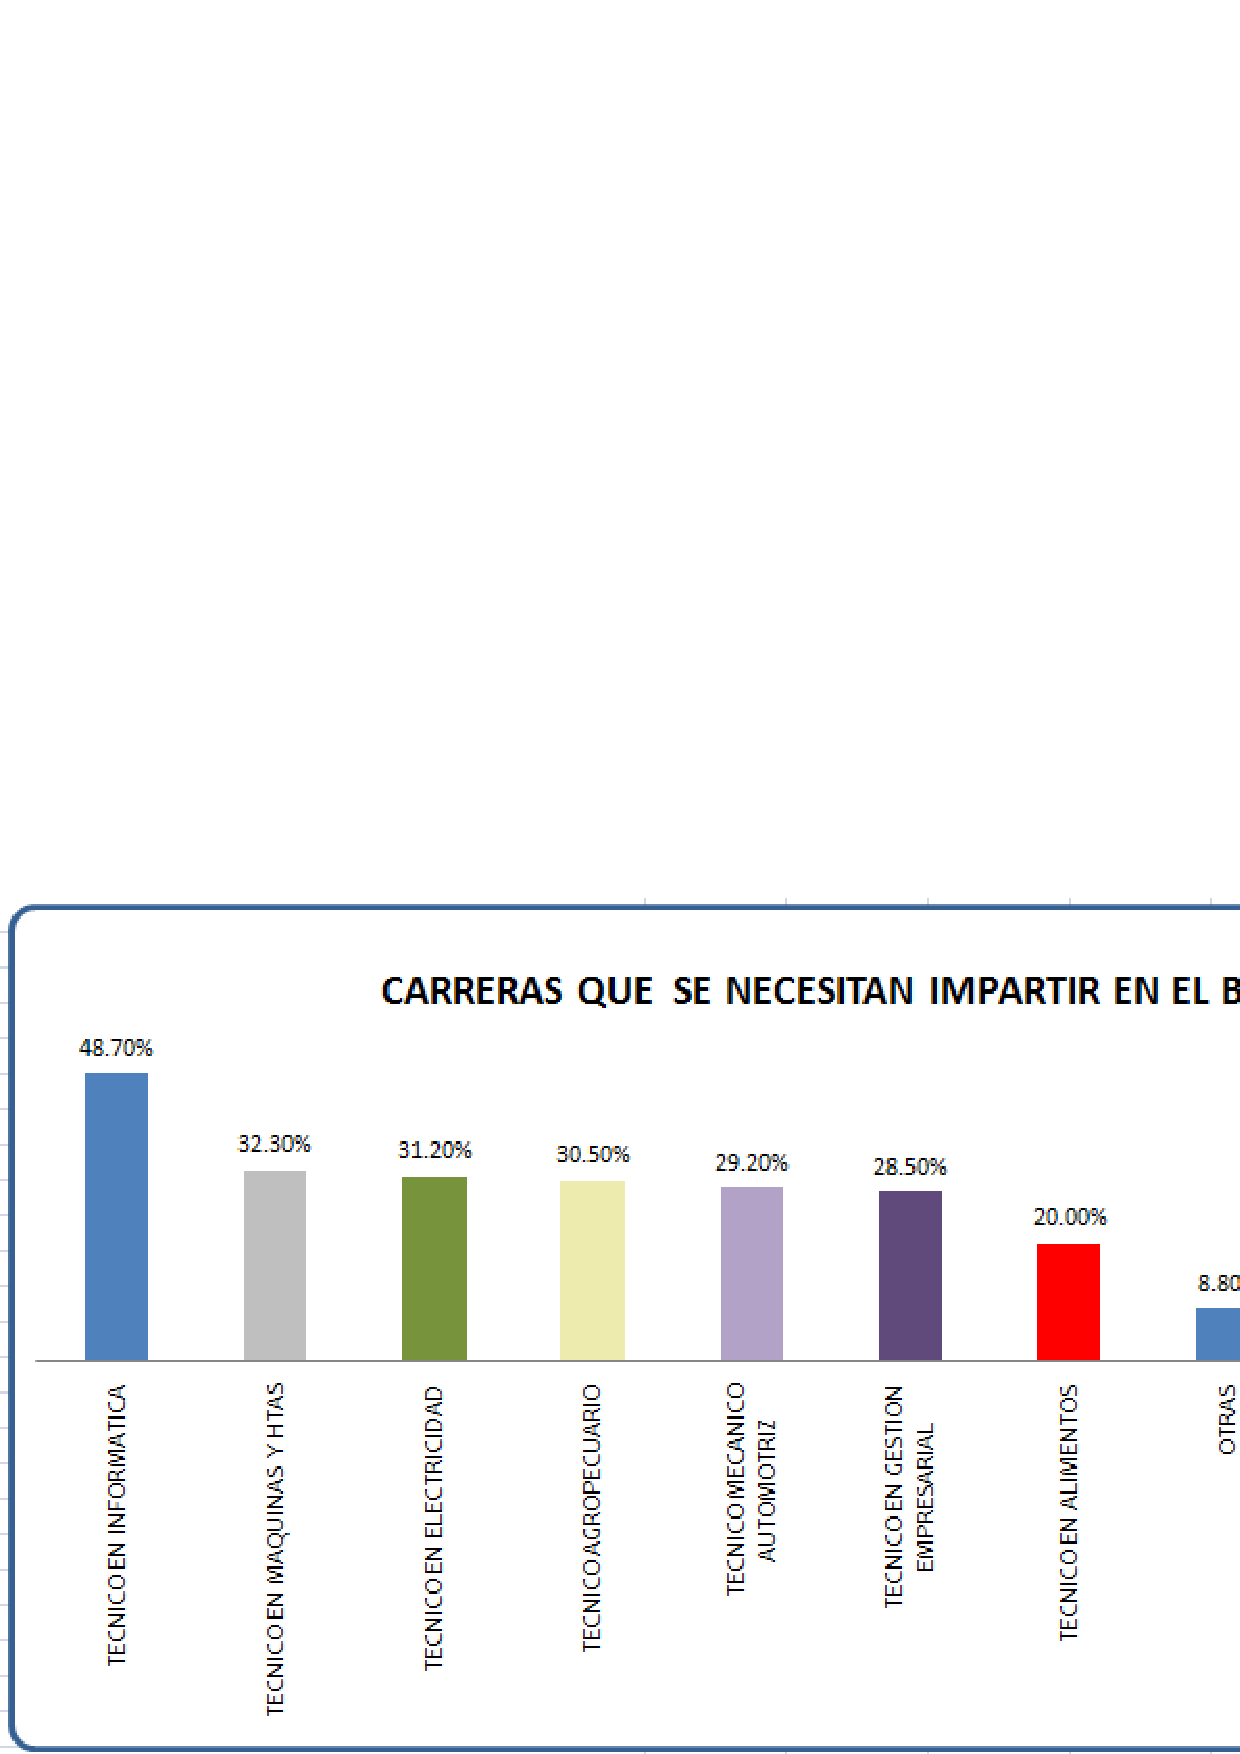
\includegraphics[scale=0.5]{images/encuesta_carreras}
	\caption{Carreras Técnicas Necesarias. Fuente: Elaboración Propia.}
	\label{fig:Encuesta:Carreras}
\end{figure}

\begin{table}[h!]
    \caption{Carreras Técnicas}
    \label{tbl:Encuesta:Carreras}
    \centering
    \begin{tabular}{@{Técnico }l|r@{.}l@{\%}}
	    \multicolumn{1}{c|}{Carrera Técnica} &
	    	\multicolumn{2}{c}{Porcentaje} \\
	    \hline
	    \hline
        en Informática                     & 48 & 70 \\
        en Máquinas y Herramientas         & 32 & 30 \\
        en Electricidad                    & 31 & 20 \\
        Agropecuario                       & 30 & 50 \\
        Mecánico Automotriz                & 29 & 20 \\
        en Gestión Empresarial             & 28 & 50 \\
        en Alimentos                       & 20 & 00 \\
        \multicolumn{1}{l|}{No especifica} &  8 & 80 \\
        \multicolumn{1}{l|}{Otras}         &  5 & 50 \\
	    \hline
	    \multicolumn{3}{l}{\footnotesize Fuente: Elaboración Propia, 2011.}
    \end{tabular}
\end{table}


\clearpage
\subsection{Posibilidad de Inscripción al Instituto}

En esta pregunta se indaga si se inscribiría el encuestado o inscribiría a sus hijos sin especificarle una fecha determinada y los resultados fueron:

\begin{figure}[h!]
	\centering
	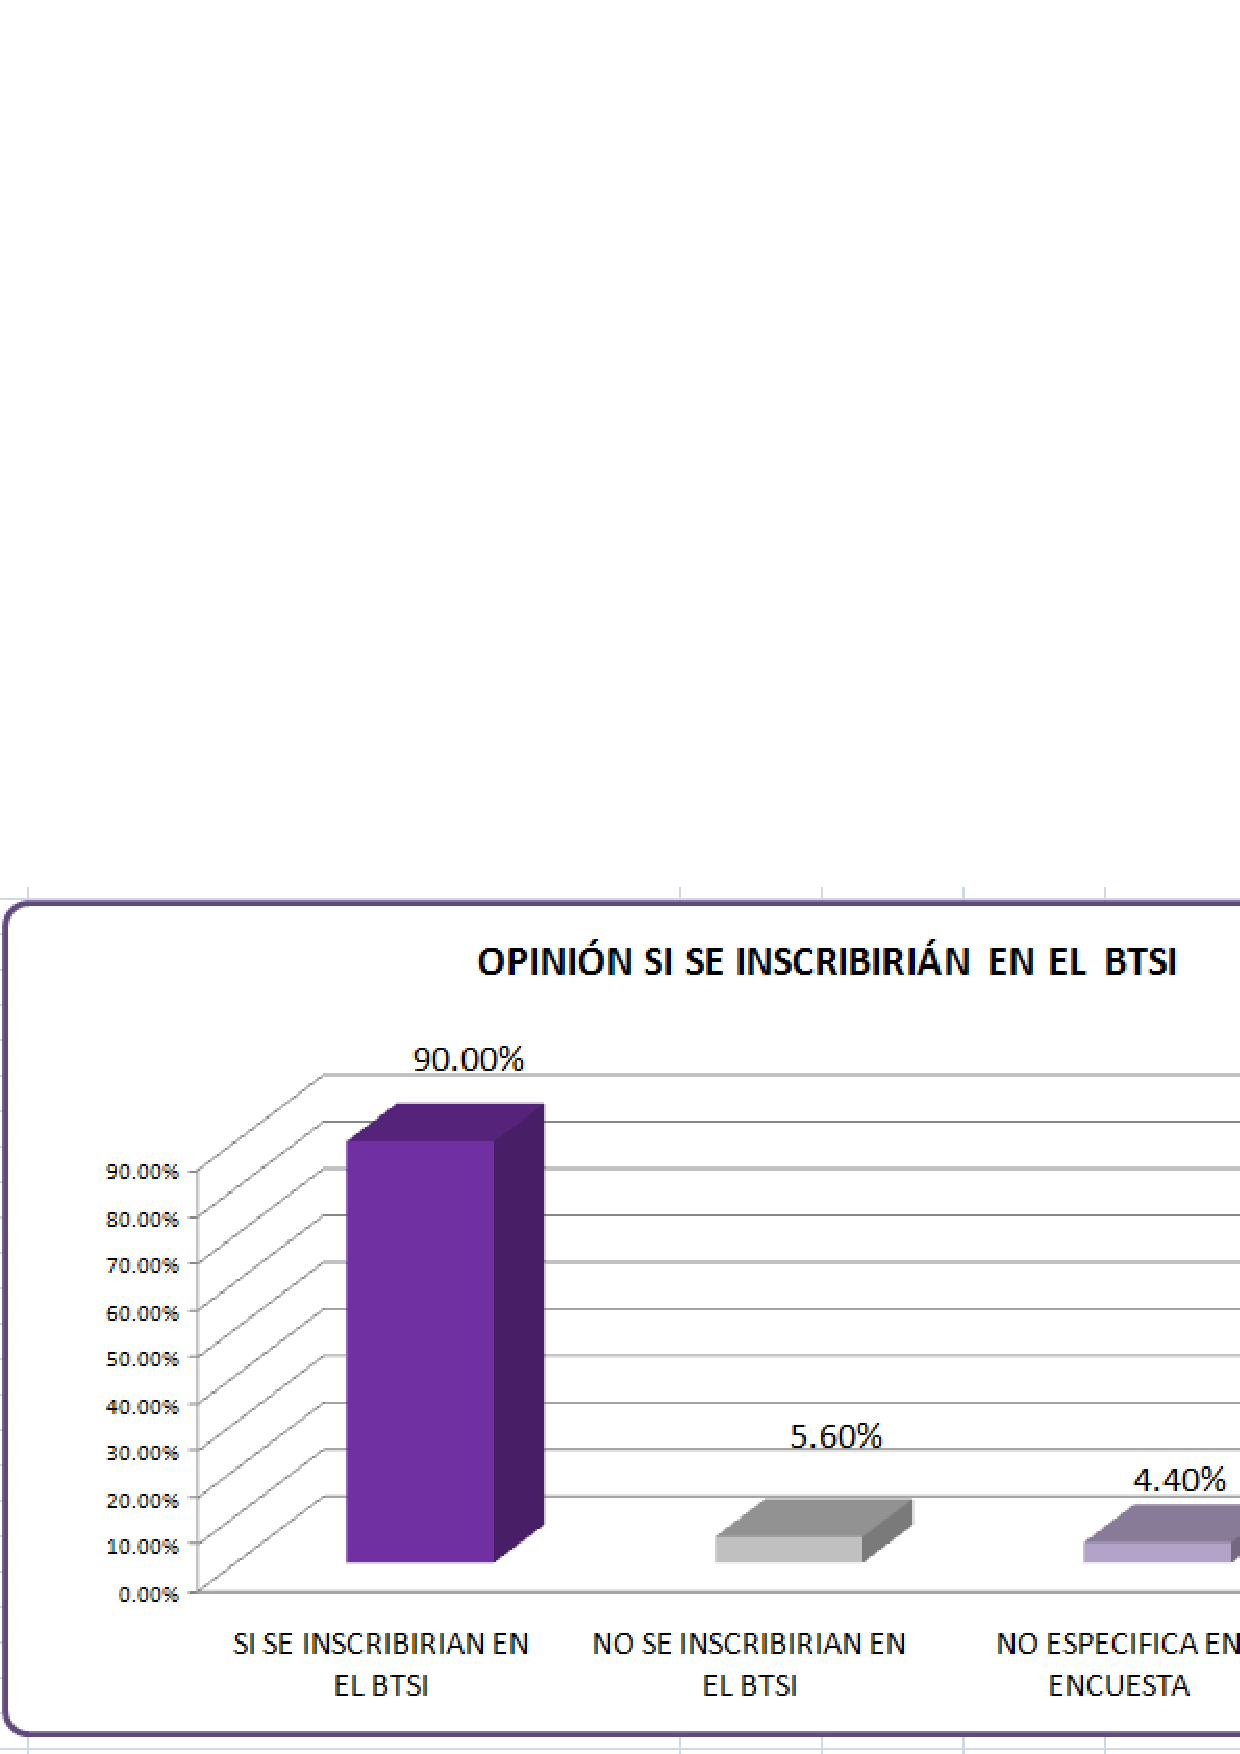
\includegraphics[scale=0.5]{images/encuesta_aceptacion}
	\caption{Posibilidad de Inscripción al Instituto. Fuente: Elaboración Propia.}
	\label{fig:Encuesta:Aceptacion}
\end{figure}

\begin{table}[h!]
    \caption{Posibilidad de Inscripción al Instituto}
    \label{tbl:Encuesta:Aceptacion}
    \centering
    \begin{tabular}{l|r@{.}l@{\%}}
	    \multicolumn{1}{c|}{Respuesta Dada} &
	    	\multicolumn{2}{c}{Porcentaje} \\
	    \hline
	    \hline
	    Sí se inscribiría en el instituto & 90 & 00 \\
	    No se inscribiría en el instituto &  5 & 60 \\
	    No lo especifica en la respuesta   &  4 & 40 \\
	    \hline
	    \multicolumn{3}{l}{\footnotesize Fuente: Elaboración Propia, 2011.}
    \end{tabular}
\end{table}


\clearpage
\subsection{Inscripciones en el Curso 2011-2012}

En esta pregunta, a diferencia de la anterior, se pregunta por la inscripción para el curso 2011-2012, y los resultados fueron:

\begin{figure}[h!]
	\centering
	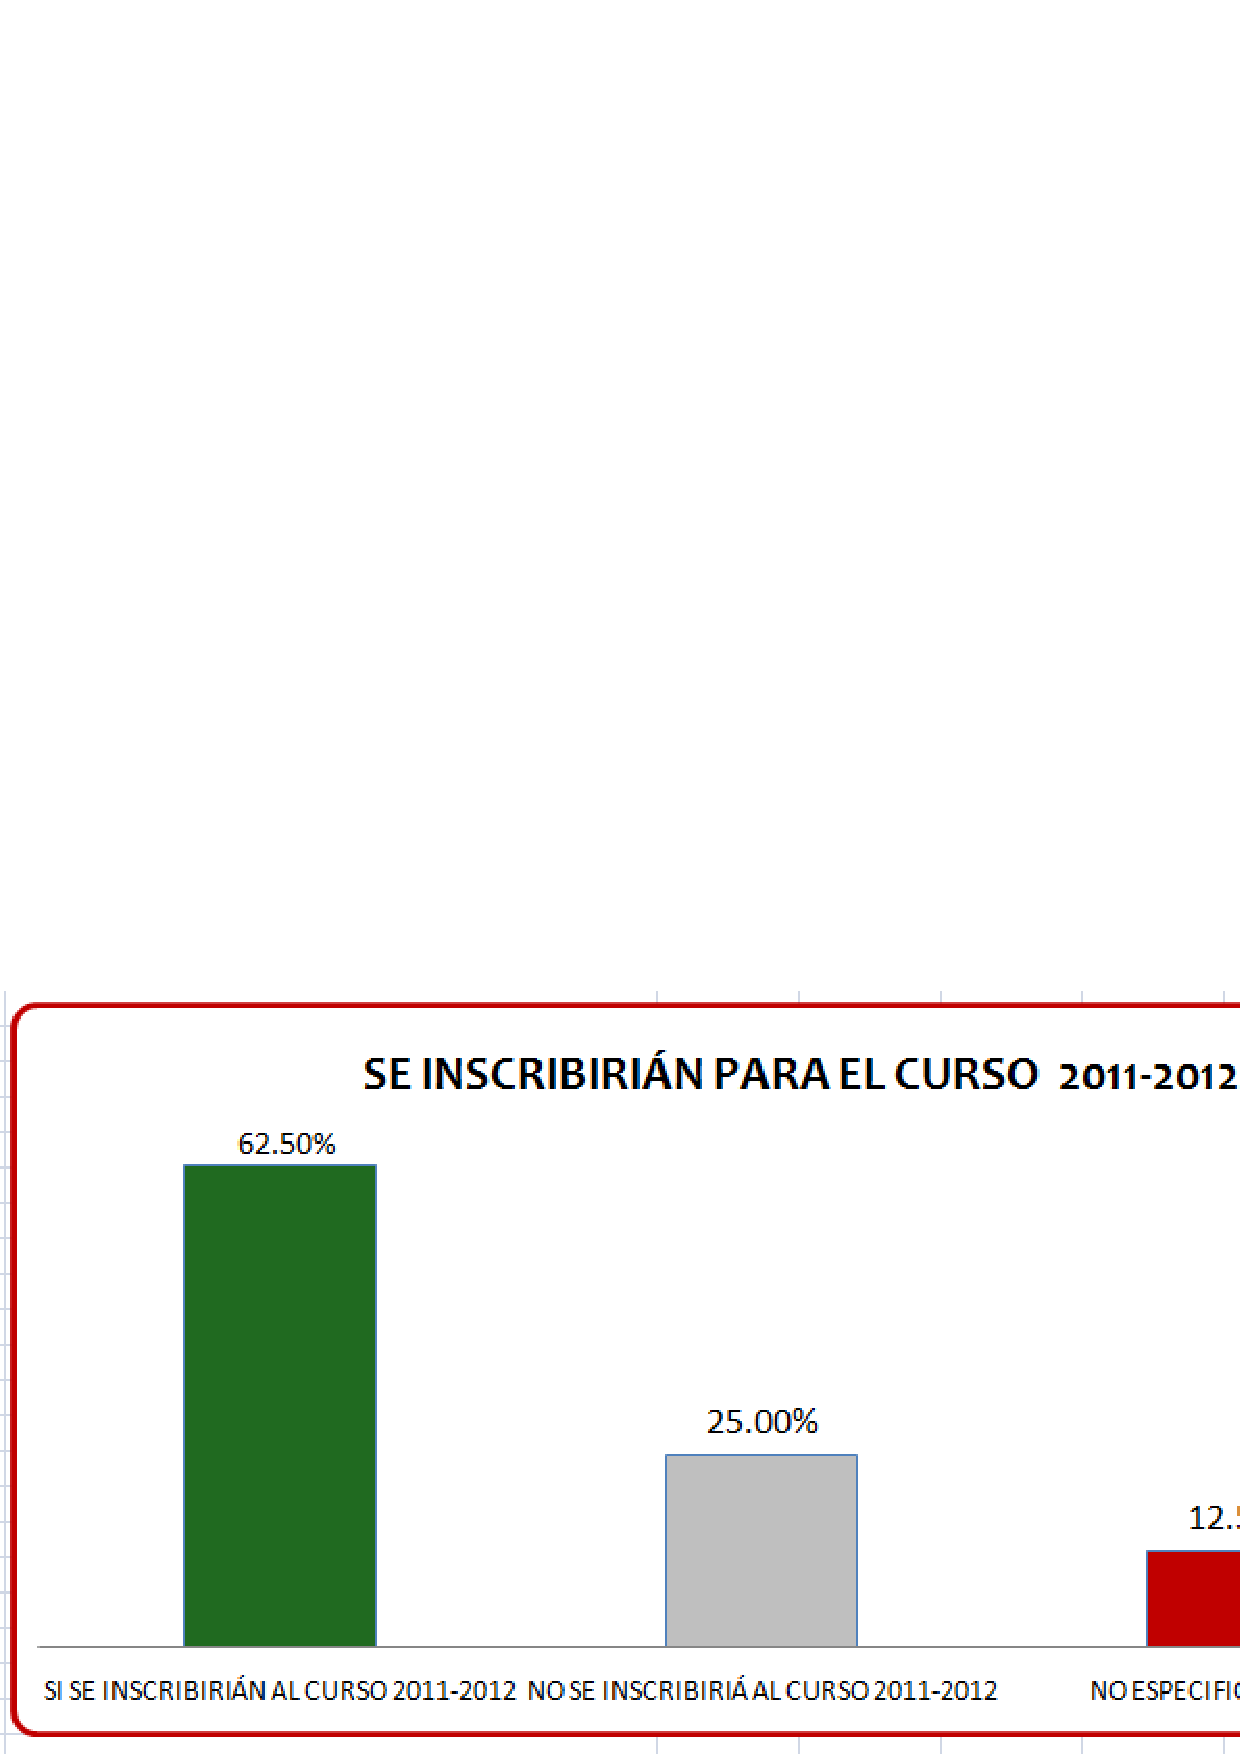
\includegraphics[scale=0.5]{images/encuesta_inscripciones_2011}
	\caption{Inscripciones en el Curso 2011-2012. Fuente: Elaboración Propia.}
	\label{fig:Encuesta:Inscripciones2011}
\end{figure}

\begin{table}[h!]
    \caption{Inscripciones en el Curso 2011-2012}
    \label{tbl:Encuesta:Inscripciones2011}
    \centering
    \begin{tabular}{l|r@{.}l@{\%}}
	    \multicolumn{1}{c|}{Respuesta Dada} &
	    	\multicolumn{2}{c}{Porcentaje} \\
	    \hline
	    \hline
	    Sí se inscribiría                  & 62 & 50 \\
	    No se inscribiría                  & 25 & 00 \\
	    No lo especifica en la respuesta   & 12 & 50 \\
	    \hline
	    \multicolumn{3}{l}{\footnotesize Fuente: Elaboración Propia, 2011.}
    \end{tabular}
\end{table}


\clearpage
\subsection{Disponibilidad de Pago}

Se pregunta a los encuestados, cuánto estarían dispuestos a pagar de colegiatura, los resultados fueron:

\begin{figure}[h!]
	\centering
	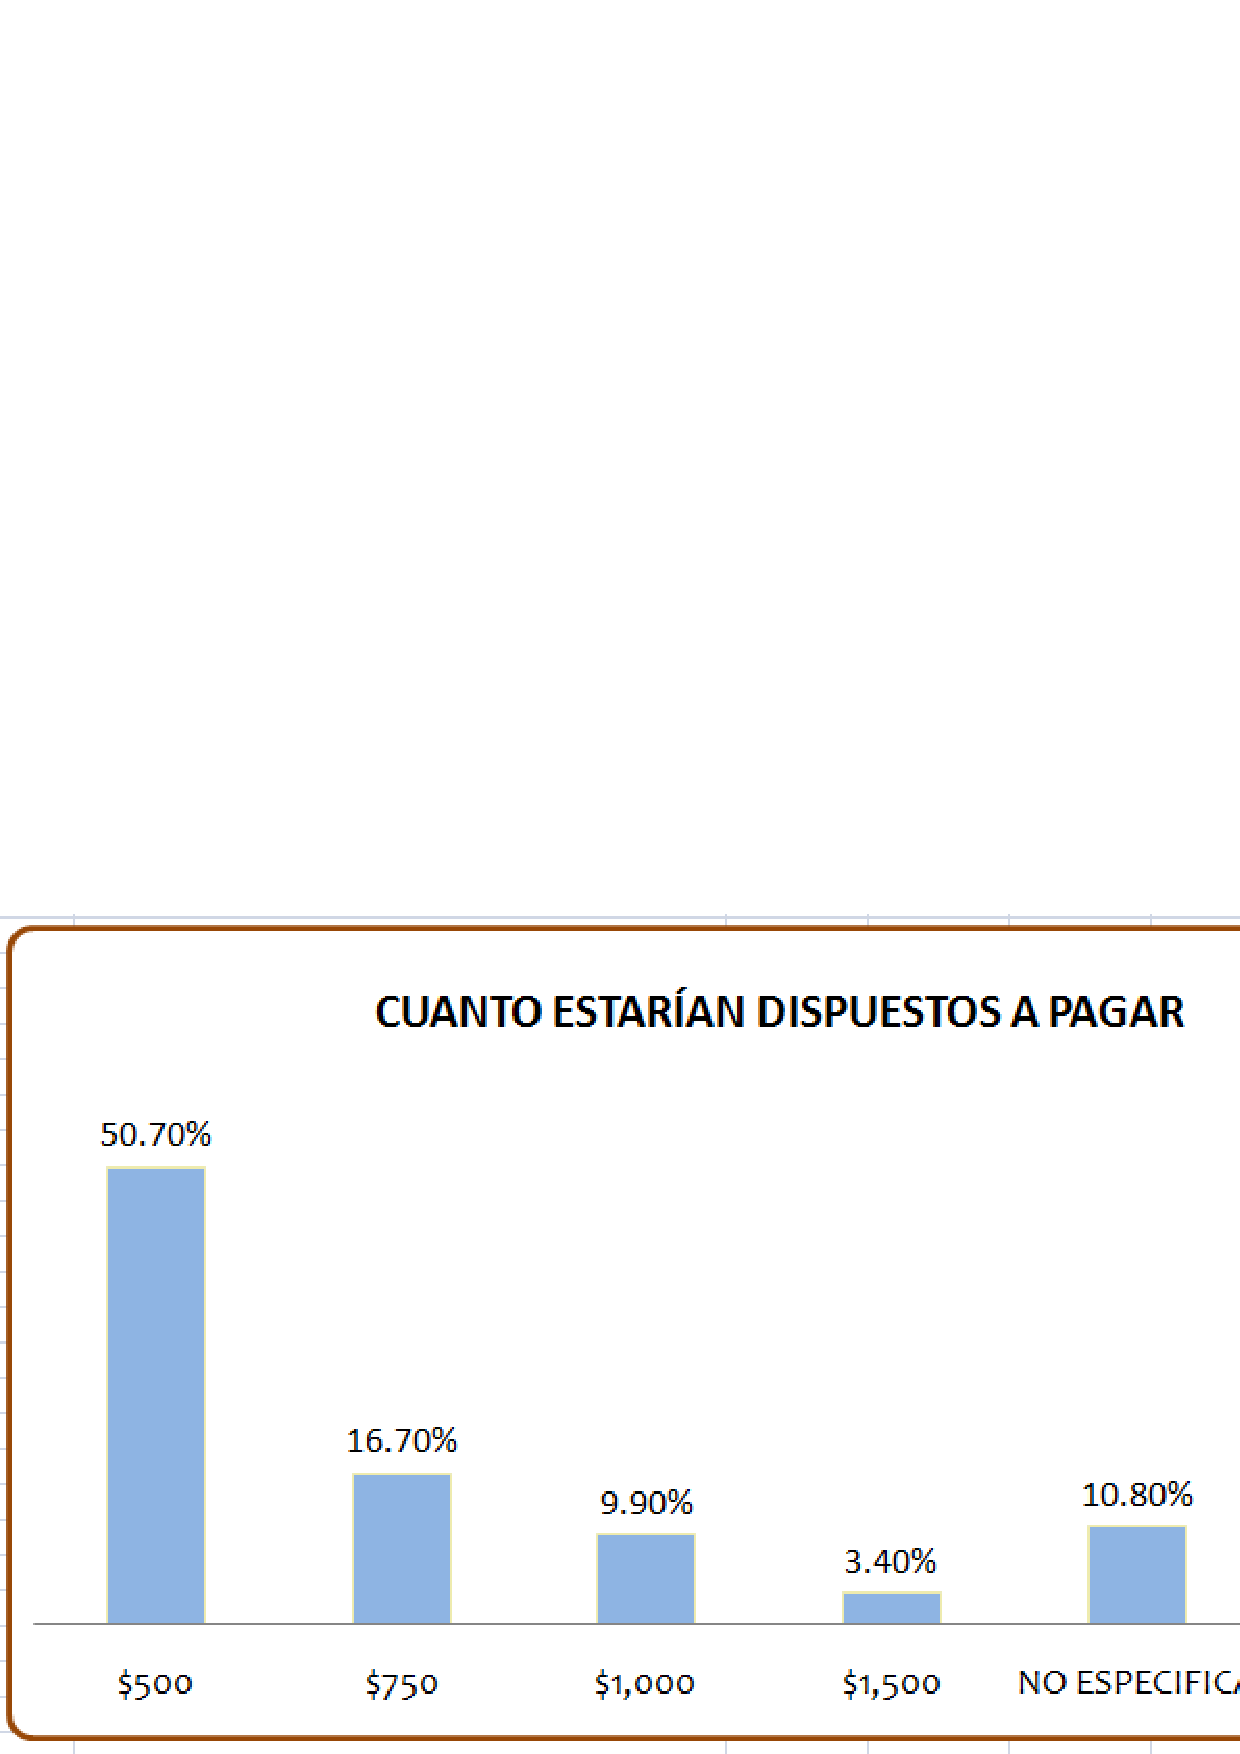
\includegraphics[scale=0.5]{images/encuesta_pago}
	\caption{Disponibilidad de Pago. Fuente: Elaboración Propia.}
	\label{fig:Encuesta:Pago}
\end{figure}

\begin{table}[h!]
    \caption{Disponibilidad de Pago}
    \label{tbl:Encuesta:Pago}
    \centering
    \begin{tabular}{@{\$ }r@{.00}|r@{.}l@{\%}}
	    \multicolumn{1}{c|}{Monto} &
	    	\multicolumn{2}{c}{Porcentaje} \\
	    \hline
	    \hline
	    500                                & 50 & 70 \\
	    750                                & 16 & 70 \\
	    1,000                              &  9 & 90 \\
	    1,500                              &  3 & 40 \\
	    \multicolumn{1}{l|}{No Especifica} & 10 & 80 \\
	    \multicolumn{1}{l|}{Otra Cantidad} &  8 & 50 \\
	    \hline
	    \multicolumn{3}{l}{\footnotesize Fuente: Elaboración Propia, 2011.}
    \end{tabular}
\end{table}



\newpage
\section{Texto Original de la Encuesta}
\begin{quote}
Proyecto Bachillerato Tecnológico Matutino en Irapuato.

\footnotesize
¡Hola! Los Salesianos de San Juan Bosco tenemos el Proyecto de un Bachillerato Tecnológico  para adolescentes  y jóvenes ofreciéndoles una educación de calidad en la formación cristiana, científica y tecnológica con la pedagogía de Don Bosco en las instalaciones del  Centro Juvenil Salesiano.

Nos gustaría conocer  tu opinión contestando estas preguntas: (Marca con una X tu respuesta)

Terminaste:
\begin{verbatim}
    a.- Primaria
    b.- Secundaria
    c.- Preparatoria
    d.- Profesión:_____________________________
Vives en la colonia:____________________________________
\end{verbatim}

1.- ¿Crees que aquí  hace falta una escuela con estas características?
\begin{verbatim}
    Sí ____ No ____
    ¿Por qué? _____________________________________________________________________
\end{verbatim}

2.- ¿Qué Carreras Técnicas crees que se necesitan?
\begin{verbatim}
    a.- Técnico en Informática       e.- Técnico en Gestión Empresarial
    b.- Técnico en Electricidad      f.- Técnico Agropecuario
    c.- Técnico en Alimentos         g.- Técnico en Máquinas y Herramientas
    d.- Técnico Mecánico Automotriz  h.- Otra _____________________________
\end{verbatim}

3.- ¿Inscribirías a tu hija o hijo en ella o te Inscribirías tú?
\begin{verbatim}
    Si ____ No ____
\end{verbatim}

4.- ¿Cuánto  podrías pagar?
\begin{verbatim}
    a.- 500 pesos  b.- 750 pesos  c.- 1000 pesos  d.- 1500  pesos  Otra________            
\end{verbatim}

5.- ¿Te inscribirías al Primer Semestre para el curso 2011-2012
\begin{verbatim}
    Sí ____ No ____
\end{verbatim}

Esperamos tu respuesta a más tardar el viernes 11 de marzo de este año a:

Francisco  Sarabia No.  511

\begin{center}
¡Los Salesianos te agradecemos ¡
\end{center}

\begin{flushright}
Irapuato,  Gto  01 Marzo de 2011.
\end{flushright}
\end{quote}
